% !TeX spellcheck = nl_NL
\documentclass{article}
\usepackage{hyperref}
\usepackage{graphicx}
\usepackage{listings}
\title{Project ComputerSystemen}
\author{Arno De Witte \\Wout Van Riel  \\Email: \href{mailto:Arno.De.Witte@vub.ac.be}{Arno.De.Witte@vub.ac.be} \\ \href{mailto:Wout.Van.Riel@vub.ac.be}{Wout.Van.Riel@vub.ac.be} \\ %i assume da da u email is
Vrije Universiteit Brussel}
\date{6 januari 2014}
\begin{document}
\maketitle
\newpage
\tableofcontents
\newpage


\section{Voorwoord}
Dit spel is gemaakt als project voor het vak Computersystemen.
Het project had als opdracht een spel te maken of een decoder voor een bepaalde encodering.
Het spel had meteen de aandacht en we begonnen na te denken over welke klassieker we zouden maken tijdens ons project.
Aangezien onze kennis van (masm) assembly niet al te groot was bij aanvang van het project, beseften we dat het spel in een 2D-omgeving gespeeld zou worden.
Space-invader was aanlokkelijk, maar niet origineel dus kregen we het idee om een avatar tegenkomende obstakels te laten ontwijken en de dit object de kans te geven om deze obstakels uit te schakelen door op hen te schieten.
We hadden al eerder spellen gezien met een gelijkaardig thema en het trok ons wel aan. Dus maakten we het spel Asteroid Field.

\section{Het spel}\label{spel}

Het concept van het spel is eenvoudig: probeer niet geraakt te worden door de asteroiden die naar de ruimtesonde komen.
Een asteroide wordt nooit op dezelfde plaats gecreëerd waardoor het spel telkens een andere ervaring is.
Om het niet eentonig en simpel te houden, zijn er levels ge\"implementeerd die na een bepaalde tijd verhogen.
Dus hoe langer de ruimtesonde kan overleven in het asteroideveld, hoe moeilijker de levels worden.
De score staat los van de levels, maar is wel aan een ander, minder logisch, aspect van het spel gekoppeld.
Elk punt dat je scoort is goed voor \'e\'en kogel dat je kan afvuren.
Wanneer de score op nul staat, is het enigste wat je kan doen de asteroiden vingervlug ontwijken en hopen dat je toch toevallig een asteroide hebt geraakt met een verdwaalde kogel.
Voor elke asteroide dat geraakt kan worden met een kogel, worden er drie punten bij de totaalscore geteld en voor elke kogel dat afgevuurd wordt, trekt het spel \'e\'en punt van de totaalscore af.
Wie een hoge score wil, kan dus beter al zijn kogels goed gebruiken.
Wanneer je geraakt wordt, zal het scherm rood flitsen.

\section{Besturing}

Het spel heeft maar drie toetsen nodig om gespeeld te worden. Namelijk de drie pijltjes: omhoog, omlaag en rechts.
Om het schip omhoog te laten gaan, moet de omhoogpijl van het toetsenbord ingedrukt worden.
Om een kogel af te vuren, moet de rechts-pijl ingedrukt worden.
Voor je begint wordt je begroet met een start scherm. Je kan het spel dan starten met de enter toets. 
Je kan het spel op elk moment verlaten met de escape toets. Je komt dan terug op de commando lijn van dosbox.

\section{Code}
De code is opgedeelt in een aantal bestanden: Game\ref{game_asm}, drawp, sprites, keyb, rand en video. Elk bestand heeft een MASM broncode bestand (.asm) en een include bestand (.inc).
Voor dit project hebben we ons gebasseerd op het gegeven code voorbeeld op pointcarr\'e. Dit wil zeggen dat we de game-loop, keyboard handling en video procedures hebben overgenomen. 
Dit was een goede basis vermits we niet meer zelf in het "lager" gelegen werk (zoals de interupts) moesten duiken en ons konden focussen op de code die belangrijk was voor het spel zelf.

\subsection{GAME.ASM}\label{game_asm}
In dit bestand bevinden zich alle data die belangrijk is voor het lopen van het spel zelf. Je vindt er bijvoorbeeld de array met obstakels en de array met beams.
Het bevat ook de main procedure die wordt opgeroepen wanneer het spel wordt uitegevoerd. Hierin bevindt zich dan ook de main loop. Deze stelt 1 cyclus van het spel voor.
Zolang er niet op escape wordt gedrukt is dit een oneindige lus. Voor de lus wordt alles geïnitialiseerd. Tijdens de lus worden de 2 belangrijkste procedures opgeroepen: renderWorld en updateWorld. 
Verder wordt er ook nog gechecked of de speler niet dood is want dan moet er niet meer worden geupdated.
RenderWorld gaat alle elementen ven het spel tekenen, terwijl updateWorld ervoor zorgt dat alle posities worden bijgewerkt. 


\section{Problemen tijdens het programmeren}\label{problems}
\begin {itemize}
\item Obstakels werden gedeeltelijk bovenaan en gedeeltelijk onderaan getekend waardoor de avatar een botsing waarneemde waneer er geen was.
\end {itemize}

\section{Screenshots}\label{screens}
\begin{figure}[htbp]
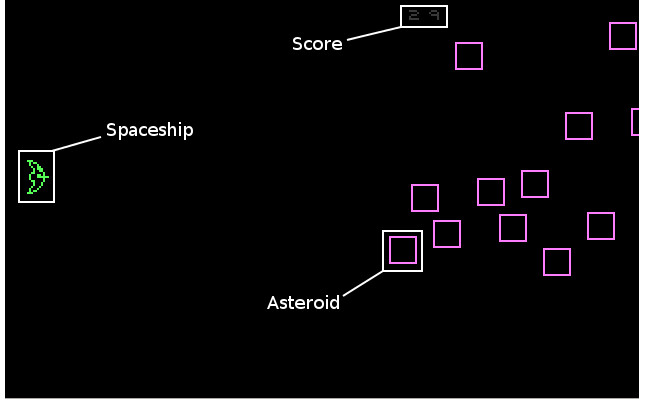
\includegraphics[width=60mm]{In_Game.jpg}
\caption{Wanneer je aan het spelen bent.}
\label{fig:ingame}
\end{figure}

\begin{figure}[htbp]
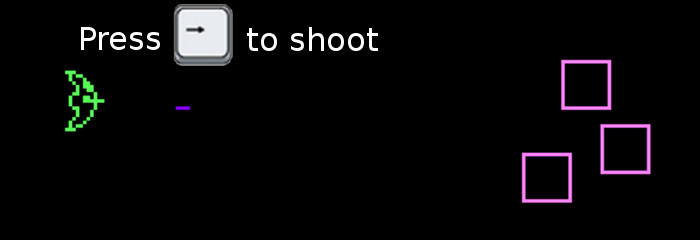
\includegraphics[width=60mm]{PressToShoot.jpg}
\caption{De besturing van het spel}
\label{fig:besturing}
\end{figure}

\begin{figure}[htbp]
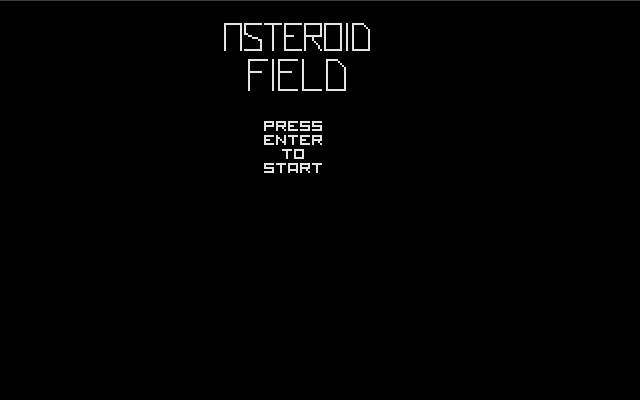
\includegraphics[width=60mm]{Menu.jpg}
\caption{Startscherm}
\label{fig:menu}
\end{figure}

\end{document}
